\documentclass[11pt,a4paper]{article}
\usepackage[utf8]{inputenc}
\usepackage[italian]{babel}
\usepackage{amsmath}
\usepackage{amsfonts}
\usepackage{amssymb}
\usepackage{graphicx}
\usepackage{minted}
\usepackage[left=2cm,right=2cm,top=2cm,bottom=2cm]{geometry}
\author{\Large Davide Grazzani}
\title{\Huge \Huge Progetto Reti Logiche}
\date{}
\begin{document}
    \maketitle
    \newpage

    \tableofcontents
    \newpage

    \section{Codifiche Convoluzionali e Introduzione al Progetto}
    Una codifica convoluzionale è un tipo di codifica utilizzata per la \textit{Forward Error Correction} (FEC) in sistemi di telecomunicazioni basati su canali monodirezionali. \\
    Quindi un codice generato da una codifica convoluzionale, detto anche codice convoluzionale, è un codice che trasforma ogni parola $P_1$ in una parola $P_2$. Definite $l_1 = lenght(P_1)$ e $l_2 = lenght(P_2)$ si definisce il rapoorto $l_1/l_2$ come \textit{tasso di trasmissione del convolutore} (rate); $l_2 \geq l_1$.\
    Inoltre la trasformazione è una funzione degli ultimi $k$ bit in entrata, $k$ è quindi la \textit{lunghezza dei vincoli} del codice.\\
    Lo scopo del progetto è quello di implementare un componente hardware, tramite l'utilizzo del linguaggio di specifica dello hardware VHDL, in grado di interfacciarsi con una memoria ram e di applicare una codifica convoluzionale con $rate = \frac{1}{2}$ e $k = 3$.
    \begin{figure}[h]
        \centering
        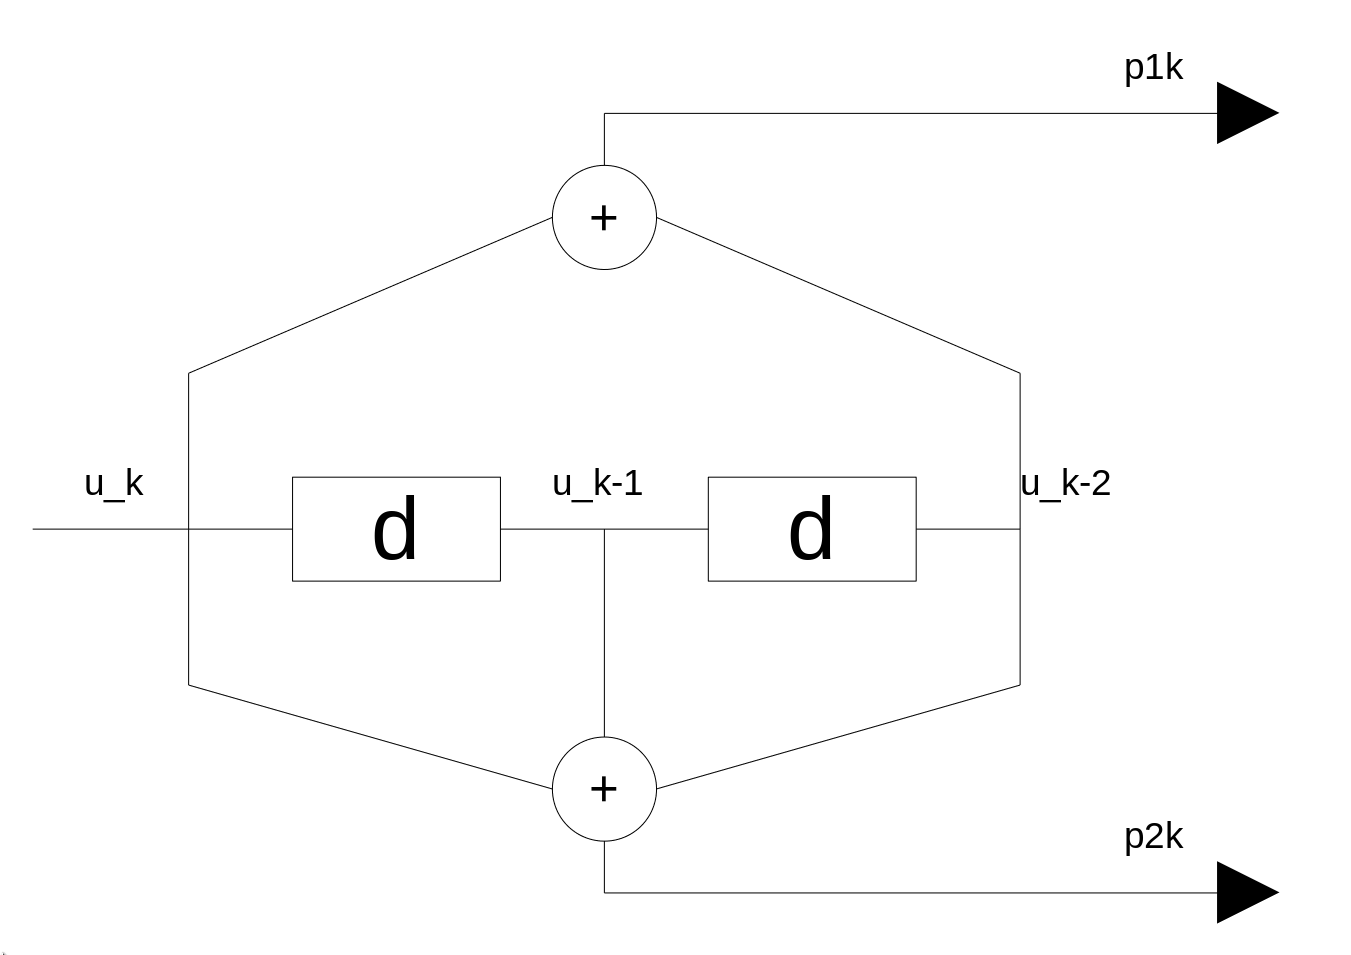
\includegraphics[width = 0.5\linewidth]{convolutore_image.png}
        \caption{Codificatore convoluzionale con $r = \frac{1}{2}$ e $k = 3$}
        \label{codificatore_convoluzionale_image}
    \end{figure}
    \subsection{Specifiche del progetto}
        Di seguito viene riportata l'interfaccia del modulo hardware da sviluppare, l'interfaccia della memoria ed infine alcune specifiche progettuali.
        \subsubsection{Interfaccia del progetto}
            \begin{minted}{vhdl}
            entity project_reti_logiche is
                port (
                    i_clk : in std_logic;
                    i_rst : in std_logic;
                    i_start : in std_logic;
                    i_data : in std_logic_vector(7 downto 0);
                    o_address : out std_logic_vector(15 downto 0);
                    o_done : out std_logic;
                    o_en : out std_logic;
                    o_we : out std_logic;
                    o_data : out std_logic_vector (7 downto 0)
                );
            end project_reti_logiche;
            \end{minted}
        \subsubsection{Interfaccia della memoria}
        TODO SISTEMARE QUESTA PARTE
        \subsubsection{Altri constrains progettuali}
        \begin{description}
            \item[Periodo di clock minimo richiesto] $clockPeriod_{req} = 100ns$
            \item[Ram] vedere   
        \end{description}
    \section{Architettura, approccio e scielte implementative}
        In questa sezione verrà descritta la \textit{FSM} del progetto seguita da un rapido overview sul codice presentato. Prima però vengono riportate alcune doverose considerazioni
        riguardanti il linguaggio di programmazione VHDL.
        \subsection{Considerazioni su VHDL}
            In questo progetto, durante la fase di progettazione e successivamente di sviluppo, non verrà preso mai in considerazione l'utilizzo del costrutto \textit{process} e di conseguenza
             di architetture di tipo \textit{behavioral} . Questa scelta implementativa, che si riflette sia in fase di sintesi che di implementazione, \underline{non è dovuta} al fatto che l'autore 
             del progetto creda che l'utilizzo di \textit{process} sia scorretto in qual si voglia forma o maniera; qui si vogliono riconoscere le potenzialità e le funzionalità implementative/strutturali 
             che ne derivano dall'utilizzo di quest'ultimi ma si vuole anche risaltare il maggior strato di astrazione portato da questo costrutto rispetto ad architetture \textit{dataflow} o \textit{structural} (aumento presumibilmente
             dovuto alle serializzazione di istuzioni che per natura fisica di un componente hardware dovrebbero essere paralle).\\
            È per il motivo sopra citato e per la non diretta corrispondenza tra codice scritto e struttura interna del sintetizzato hardware che in questo progetto sono state scartate implementazioni di tipo \textit{behavioral}.
        \subsection{Primo design della FSM}
            Tenendo conto delle considerazioni sopra fatte viene ora presentata la prima macchina a stati in grado già di soddisfare ampiamente requisiti di timing sia post sintesi sia post implementazione; viene discussa quest'ultima in 
            quanto alla base del design finale e da considerarsi design ottimale per periodi di clock $clockPeriod \approx [35,100] ns$\\
            TODO disegno della macchina a stati 
            \subsubsection{Stati della macchina}
            
\end{document}